% Created by tikzDevice version 0.12.6 on 2024-02-18 17:32:29
% !TEX encoding = UTF-8 Unicode
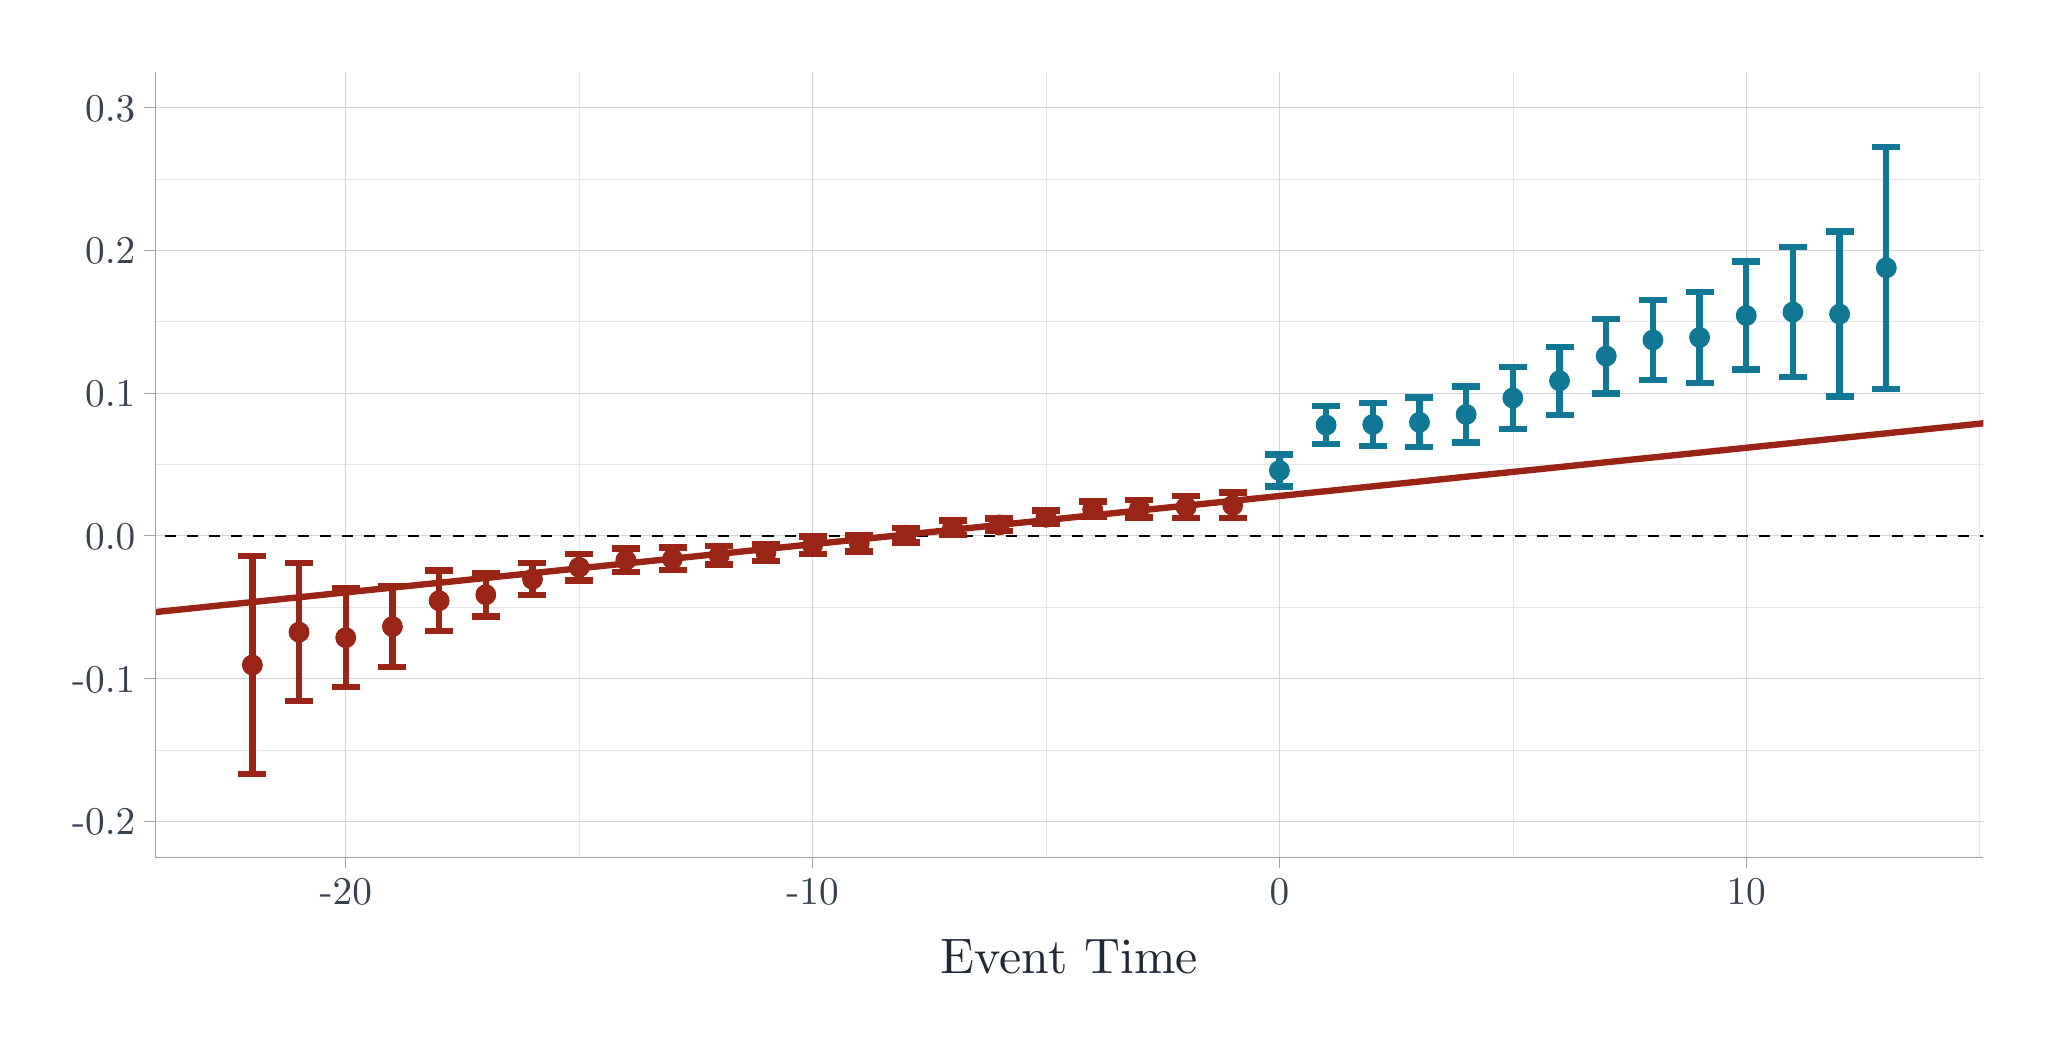
\begin{tikzpicture}[x=1pt,y=1pt]
\definecolor{fillColor}{RGB}{255,255,255}
\path[use as bounding box,fill=fillColor] (0,0) rectangle (722.70,361.35);
\begin{scope}
\path[clip] (  0.00,  0.00) rectangle (722.70,361.35);
\definecolor{drawColor}{RGB}{255,255,255}

\path[draw=drawColor,line width= 0.8pt,line join=round,line cap=round,fill=fillColor] (  0.00,  0.00) rectangle (722.70,361.35);
\end{scope}
\begin{scope}
\path[clip] ( 46.10, 61.65) rectangle (706.70,345.35);
\definecolor{drawColor}{RGB}{255,255,255}
\definecolor{fillColor}{RGB}{255,255,255}

\path[draw=drawColor,line width= 0.8pt,line join=round,line cap=round,fill=fillColor] ( 46.10, 61.65) rectangle (706.70,345.35);
\definecolor{drawColor}{RGB}{229,231,235}

\path[draw=drawColor,line width= 0.2pt,line join=round] ( 46.10,100.34) --
	(706.70,100.34);

\path[draw=drawColor,line width= 0.2pt,line join=round] ( 46.10,151.92) --
	(706.70,151.92);

\path[draw=drawColor,line width= 0.2pt,line join=round] ( 46.10,203.50) --
	(706.70,203.50);

\path[draw=drawColor,line width= 0.2pt,line join=round] ( 46.10,255.08) --
	(706.70,255.08);

\path[draw=drawColor,line width= 0.2pt,line join=round] ( 46.10,306.66) --
	(706.70,306.66);

\path[draw=drawColor,line width= 0.2pt,line join=round] (199.28, 61.65) --
	(199.28,345.35);

\path[draw=drawColor,line width= 0.2pt,line join=round] (367.97, 61.65) --
	(367.97,345.35);

\path[draw=drawColor,line width= 0.2pt,line join=round] (536.66, 61.65) --
	(536.66,345.35);

\path[draw=drawColor,line width= 0.2pt,line join=round] (705.35, 61.65) --
	(705.35,345.35);
\definecolor{drawColor}{RGB}{209,213,219}

\path[draw=drawColor,line width= 0.4pt,line join=round] ( 46.10, 74.55) --
	(706.70, 74.55);

\path[draw=drawColor,line width= 0.4pt,line join=round] ( 46.10,126.13) --
	(706.70,126.13);

\path[draw=drawColor,line width= 0.4pt,line join=round] ( 46.10,177.71) --
	(706.70,177.71);

\path[draw=drawColor,line width= 0.4pt,line join=round] ( 46.10,229.29) --
	(706.70,229.29);

\path[draw=drawColor,line width= 0.4pt,line join=round] ( 46.10,280.87) --
	(706.70,280.87);

\path[draw=drawColor,line width= 0.4pt,line join=round] ( 46.10,332.45) --
	(706.70,332.45);

\path[draw=drawColor,line width= 0.4pt,line join=round] (114.93, 61.65) --
	(114.93,345.35);

\path[draw=drawColor,line width= 0.4pt,line join=round] (283.62, 61.65) --
	(283.62,345.35);

\path[draw=drawColor,line width= 0.4pt,line join=round] (452.31, 61.65) --
	(452.31,345.35);

\path[draw=drawColor,line width= 0.4pt,line join=round] (621.00, 61.65) --
	(621.00,345.35);
\definecolor{drawColor}{RGB}{0,0,0}

\path[draw=drawColor,line width= 0.9pt,dash pattern=on 4pt off 4pt ,line join=round] (-614.49,177.71) -- (1367.30,177.71);
\definecolor{drawColor}{RGB}{154,36,21}

\path[draw=drawColor,line width= 2.3pt,line join=round] (-614.49, 81.94) -- (1367.30,286.61);
\definecolor{fillColor}{RGB}{154,36,21}

\path[draw=drawColor,line width= 0.4pt,line join=round,line cap=round,fill=fillColor] ( 81.19,131.04) circle (  3.57);

\path[draw=drawColor,line width= 0.4pt,line join=round,line cap=round,fill=fillColor] ( 98.06,142.93) circle (  3.57);

\path[draw=drawColor,line width= 0.4pt,line join=round,line cap=round,fill=fillColor] (114.93,140.92) circle (  3.57);

\path[draw=drawColor,line width= 0.4pt,line join=round,line cap=round,fill=fillColor] (131.80,144.92) circle (  3.57);

\path[draw=drawColor,line width= 0.4pt,line join=round,line cap=round,fill=fillColor] (148.67,154.27) circle (  3.57);

\path[draw=drawColor,line width= 0.4pt,line join=round,line cap=round,fill=fillColor] (165.54,156.44) circle (  3.57);

\path[draw=drawColor,line width= 0.4pt,line join=round,line cap=round,fill=fillColor] (182.41,162.06) circle (  3.57);

\path[draw=drawColor,line width= 0.4pt,line join=round,line cap=round,fill=fillColor] (199.28,166.35) circle (  3.57);

\path[draw=drawColor,line width= 0.4pt,line join=round,line cap=round,fill=fillColor] (216.15,168.93) circle (  3.57);

\path[draw=drawColor,line width= 0.4pt,line join=round,line cap=round,fill=fillColor] (233.01,169.37) circle (  3.57);

\path[draw=drawColor,line width= 0.4pt,line join=round,line cap=round,fill=fillColor] (249.88,170.68) circle (  3.57);

\path[draw=drawColor,line width= 0.4pt,line join=round,line cap=round,fill=fillColor] (266.75,171.63) circle (  3.57);

\path[draw=drawColor,line width= 0.4pt,line join=round,line cap=round,fill=fillColor] (283.62,174.30) circle (  3.57);

\path[draw=drawColor,line width= 0.4pt,line join=round,line cap=round,fill=fillColor] (300.49,175.03) circle (  3.57);

\path[draw=drawColor,line width= 0.4pt,line join=round,line cap=round,fill=fillColor] (317.36,177.95) circle (  3.57);

\path[draw=drawColor,line width= 0.4pt,line join=round,line cap=round,fill=fillColor] (334.23,180.71) circle (  3.57);

\path[draw=drawColor,line width= 0.4pt,line join=round,line cap=round,fill=fillColor] (351.10,181.66) circle (  3.57);

\path[draw=drawColor,line width= 0.4pt,line join=round,line cap=round,fill=fillColor] (367.97,184.43) circle (  3.57);

\path[draw=drawColor,line width= 0.4pt,line join=round,line cap=round,fill=fillColor] (384.84,187.27) circle (  3.57);

\path[draw=drawColor,line width= 0.4pt,line join=round,line cap=round,fill=fillColor] (401.71,187.54) circle (  3.57);

\path[draw=drawColor,line width= 0.4pt,line join=round,line cap=round,fill=fillColor] (418.58,188.13) circle (  3.57);

\path[draw=drawColor,line width= 0.4pt,line join=round,line cap=round,fill=fillColor] (435.44,188.72) circle (  3.57);
\definecolor{drawColor}{RGB}{16,120,149}
\definecolor{fillColor}{RGB}{16,120,149}

\path[draw=drawColor,line width= 0.4pt,line join=round,line cap=round,fill=fillColor] (452.31,201.31) circle (  3.57);

\path[draw=drawColor,line width= 0.4pt,line join=round,line cap=round,fill=fillColor] (469.18,217.76) circle (  3.57);

\path[draw=drawColor,line width= 0.4pt,line join=round,line cap=round,fill=fillColor] (486.05,217.94) circle (  3.57);

\path[draw=drawColor,line width= 0.4pt,line join=round,line cap=round,fill=fillColor] (502.92,218.76) circle (  3.57);

\path[draw=drawColor,line width= 0.4pt,line join=round,line cap=round,fill=fillColor] (519.79,221.59) circle (  3.57);

\path[draw=drawColor,line width= 0.4pt,line join=round,line cap=round,fill=fillColor] (536.66,227.53) circle (  3.57);

\path[draw=drawColor,line width= 0.4pt,line join=round,line cap=round,fill=fillColor] (553.53,233.76) circle (  3.57);

\path[draw=drawColor,line width= 0.4pt,line join=round,line cap=round,fill=fillColor] (570.40,242.69) circle (  3.57);

\path[draw=drawColor,line width= 0.4pt,line join=round,line cap=round,fill=fillColor] (587.27,248.49) circle (  3.57);

\path[draw=drawColor,line width= 0.4pt,line join=round,line cap=round,fill=fillColor] (604.14,249.40) circle (  3.57);

\path[draw=drawColor,line width= 0.4pt,line join=round,line cap=round,fill=fillColor] (621.00,257.33) circle (  3.57);

\path[draw=drawColor,line width= 0.4pt,line join=round,line cap=round,fill=fillColor] (637.87,258.59) circle (  3.57);

\path[draw=drawColor,line width= 0.4pt,line join=round,line cap=round,fill=fillColor] (654.74,257.86) circle (  3.57);

\path[draw=drawColor,line width= 0.4pt,line join=round,line cap=round,fill=fillColor] (671.61,274.56) circle (  3.57);
\definecolor{drawColor}{RGB}{154,36,21}

\path[draw=drawColor,line width= 2.3pt,line join=round] ( 76.13,170.40) --
	( 86.25,170.40);

\path[draw=drawColor,line width= 2.3pt,line join=round] ( 81.19,170.40) --
	( 81.19, 91.68);

\path[draw=drawColor,line width= 2.3pt,line join=round] ( 76.13, 91.68) --
	( 86.25, 91.68);

\path[draw=drawColor,line width= 2.3pt,line join=round] ( 93.00,167.88) --
	(103.12,167.88);

\path[draw=drawColor,line width= 2.3pt,line join=round] ( 98.06,167.88) --
	( 98.06,117.97);

\path[draw=drawColor,line width= 2.3pt,line join=round] ( 93.00,117.97) --
	(103.12,117.97);

\path[draw=drawColor,line width= 2.3pt,line join=round] (109.87,158.78) --
	(119.99,158.78);

\path[draw=drawColor,line width= 2.3pt,line join=round] (114.93,158.78) --
	(114.93,123.06);

\path[draw=drawColor,line width= 2.3pt,line join=round] (109.87,123.06) --
	(119.99,123.06);

\path[draw=drawColor,line width= 2.3pt,line join=round] (126.74,159.53) --
	(136.86,159.53);

\path[draw=drawColor,line width= 2.3pt,line join=round] (131.80,159.53) --
	(131.80,130.32);

\path[draw=drawColor,line width= 2.3pt,line join=round] (126.74,130.32) --
	(136.86,130.32);

\path[draw=drawColor,line width= 2.3pt,line join=round] (143.61,165.17) --
	(153.73,165.17);

\path[draw=drawColor,line width= 2.3pt,line join=round] (148.67,165.17) --
	(148.67,143.37);

\path[draw=drawColor,line width= 2.3pt,line join=round] (143.61,143.37) --
	(153.73,143.37);

\path[draw=drawColor,line width= 2.3pt,line join=round] (160.48,164.29) --
	(170.60,164.29);

\path[draw=drawColor,line width= 2.3pt,line join=round] (165.54,164.29) --
	(165.54,148.59);

\path[draw=drawColor,line width= 2.3pt,line join=round] (160.48,148.59) --
	(170.60,148.59);

\path[draw=drawColor,line width= 2.3pt,line join=round] (177.35,167.84) --
	(187.47,167.84);

\path[draw=drawColor,line width= 2.3pt,line join=round] (182.41,167.84) --
	(182.41,156.28);

\path[draw=drawColor,line width= 2.3pt,line join=round] (177.35,156.28) --
	(187.47,156.28);

\path[draw=drawColor,line width= 2.3pt,line join=round] (194.22,171.15) --
	(204.34,171.15);

\path[draw=drawColor,line width= 2.3pt,line join=round] (199.28,171.15) --
	(199.28,161.56);

\path[draw=drawColor,line width= 2.3pt,line join=round] (194.22,161.56) --
	(204.34,161.56);

\path[draw=drawColor,line width= 2.3pt,line join=round] (211.08,173.14) --
	(221.21,173.14);

\path[draw=drawColor,line width= 2.3pt,line join=round] (216.15,173.14) --
	(216.15,164.72);

\path[draw=drawColor,line width= 2.3pt,line join=round] (211.08,164.72) --
	(221.21,164.72);

\path[draw=drawColor,line width= 2.3pt,line join=round] (227.95,173.47) --
	(238.08,173.47);

\path[draw=drawColor,line width= 2.3pt,line join=round] (233.01,173.47) --
	(233.01,165.27);

\path[draw=drawColor,line width= 2.3pt,line join=round] (227.95,165.27) --
	(238.08,165.27);

\path[draw=drawColor,line width= 2.3pt,line join=round] (244.82,174.00) --
	(254.94,174.00);

\path[draw=drawColor,line width= 2.3pt,line join=round] (249.88,174.00) --
	(249.88,167.37);

\path[draw=drawColor,line width= 2.3pt,line join=round] (244.82,167.37) --
	(254.94,167.37);

\path[draw=drawColor,line width= 2.3pt,line join=round] (261.69,174.68) --
	(271.81,174.68);

\path[draw=drawColor,line width= 2.3pt,line join=round] (266.75,174.68) --
	(266.75,168.58);

\path[draw=drawColor,line width= 2.3pt,line join=round] (261.69,168.58) --
	(271.81,168.58);

\path[draw=drawColor,line width= 2.3pt,line join=round] (278.56,177.42) --
	(288.68,177.42);

\path[draw=drawColor,line width= 2.3pt,line join=round] (283.62,177.42) --
	(283.62,171.17);

\path[draw=drawColor,line width= 2.3pt,line join=round] (278.56,171.17) --
	(288.68,171.17);

\path[draw=drawColor,line width= 2.3pt,line join=round] (295.43,178.00) --
	(305.55,178.00);

\path[draw=drawColor,line width= 2.3pt,line join=round] (300.49,178.00) --
	(300.49,172.06);

\path[draw=drawColor,line width= 2.3pt,line join=round] (295.43,172.06) --
	(305.55,172.06);

\path[draw=drawColor,line width= 2.3pt,line join=round] (312.30,180.58) --
	(322.42,180.58);

\path[draw=drawColor,line width= 2.3pt,line join=round] (317.36,180.58) --
	(317.36,175.31);

\path[draw=drawColor,line width= 2.3pt,line join=round] (312.30,175.31) --
	(322.42,175.31);

\path[draw=drawColor,line width= 2.3pt,line join=round] (329.17,183.30) --
	(339.29,183.30);

\path[draw=drawColor,line width= 2.3pt,line join=round] (334.23,183.30) --
	(334.23,178.12);

\path[draw=drawColor,line width= 2.3pt,line join=round] (329.17,178.12) --
	(339.29,178.12);

\path[draw=drawColor,line width= 2.3pt,line join=round] (346.04,183.94) --
	(356.16,183.94);

\path[draw=drawColor,line width= 2.3pt,line join=round] (351.10,183.94) --
	(351.10,179.38);

\path[draw=drawColor,line width= 2.3pt,line join=round] (346.04,179.38) --
	(356.16,179.38);

\path[draw=drawColor,line width= 2.3pt,line join=round] (362.91,186.84) --
	(373.03,186.84);

\path[draw=drawColor,line width= 2.3pt,line join=round] (367.97,186.84) --
	(367.97,182.02);

\path[draw=drawColor,line width= 2.3pt,line join=round] (362.91,182.02) --
	(373.03,182.02);

\path[draw=drawColor,line width= 2.3pt,line join=round] (379.78,190.07) --
	(389.90,190.07);

\path[draw=drawColor,line width= 2.3pt,line join=round] (384.84,190.07) --
	(384.84,184.47);

\path[draw=drawColor,line width= 2.3pt,line join=round] (379.78,184.47) --
	(389.90,184.47);

\path[draw=drawColor,line width= 2.3pt,line join=round] (396.65,190.70) --
	(406.77,190.70);

\path[draw=drawColor,line width= 2.3pt,line join=round] (401.71,190.70) --
	(401.71,184.38);

\path[draw=drawColor,line width= 2.3pt,line join=round] (396.65,184.38) --
	(406.77,184.38);

\path[draw=drawColor,line width= 2.3pt,line join=round] (413.51,192.03) --
	(423.64,192.03);

\path[draw=drawColor,line width= 2.3pt,line join=round] (418.58,192.03) --
	(418.58,184.23);

\path[draw=drawColor,line width= 2.3pt,line join=round] (413.51,184.23) --
	(423.64,184.23);

\path[draw=drawColor,line width= 2.3pt,line join=round] (430.38,193.35) --
	(440.50,193.35);

\path[draw=drawColor,line width= 2.3pt,line join=round] (435.44,193.35) --
	(435.44,184.09);

\path[draw=drawColor,line width= 2.3pt,line join=round] (430.38,184.09) --
	(440.50,184.09);
\definecolor{drawColor}{RGB}{16,120,149}

\path[draw=drawColor,line width= 2.3pt,line join=round] (447.25,207.12) --
	(457.37,207.12);

\path[draw=drawColor,line width= 2.3pt,line join=round] (452.31,207.12) --
	(452.31,195.49);

\path[draw=drawColor,line width= 2.3pt,line join=round] (447.25,195.49) --
	(457.37,195.49);

\path[draw=drawColor,line width= 2.3pt,line join=round] (464.12,224.53) --
	(474.24,224.53);

\path[draw=drawColor,line width= 2.3pt,line join=round] (469.18,224.53) --
	(469.18,210.99);

\path[draw=drawColor,line width= 2.3pt,line join=round] (464.12,210.99) --
	(474.24,210.99);

\path[draw=drawColor,line width= 2.3pt,line join=round] (480.99,225.62) --
	(491.11,225.62);

\path[draw=drawColor,line width= 2.3pt,line join=round] (486.05,225.62) --
	(486.05,210.27);

\path[draw=drawColor,line width= 2.3pt,line join=round] (480.99,210.27) --
	(491.11,210.27);

\path[draw=drawColor,line width= 2.3pt,line join=round] (497.86,227.75) --
	(507.98,227.75);

\path[draw=drawColor,line width= 2.3pt,line join=round] (502.92,227.75) --
	(502.92,209.76);

\path[draw=drawColor,line width= 2.3pt,line join=round] (497.86,209.76) --
	(507.98,209.76);

\path[draw=drawColor,line width= 2.3pt,line join=round] (514.73,231.72) --
	(524.85,231.72);

\path[draw=drawColor,line width= 2.3pt,line join=round] (519.79,231.72) --
	(519.79,211.47);

\path[draw=drawColor,line width= 2.3pt,line join=round] (514.73,211.47) --
	(524.85,211.47);

\path[draw=drawColor,line width= 2.3pt,line join=round] (531.60,238.77) --
	(541.72,238.77);

\path[draw=drawColor,line width= 2.3pt,line join=round] (536.66,238.77) --
	(536.66,216.29);

\path[draw=drawColor,line width= 2.3pt,line join=round] (531.60,216.29) --
	(541.72,216.29);

\path[draw=drawColor,line width= 2.3pt,line join=round] (548.47,246.07) --
	(558.59,246.07);

\path[draw=drawColor,line width= 2.3pt,line join=round] (553.53,246.07) --
	(553.53,221.44);

\path[draw=drawColor,line width= 2.3pt,line join=round] (548.47,221.44) --
	(558.59,221.44);

\path[draw=drawColor,line width= 2.3pt,line join=round] (565.34,256.18) --
	(575.46,256.18);

\path[draw=drawColor,line width= 2.3pt,line join=round] (570.40,256.18) --
	(570.40,229.20);

\path[draw=drawColor,line width= 2.3pt,line join=round] (565.34,229.20) --
	(575.46,229.20);

\path[draw=drawColor,line width= 2.3pt,line join=round] (582.21,263.05) --
	(592.33,263.05);

\path[draw=drawColor,line width= 2.3pt,line join=round] (587.27,263.05) --
	(587.27,233.94);

\path[draw=drawColor,line width= 2.3pt,line join=round] (582.21,233.94) --
	(592.33,233.94);

\path[draw=drawColor,line width= 2.3pt,line join=round] (599.07,265.84) --
	(609.20,265.84);

\path[draw=drawColor,line width= 2.3pt,line join=round] (604.14,265.84) --
	(604.14,232.96);

\path[draw=drawColor,line width= 2.3pt,line join=round] (599.07,232.96) --
	(609.20,232.96);

\path[draw=drawColor,line width= 2.3pt,line join=round] (615.94,276.84) --
	(626.07,276.84);

\path[draw=drawColor,line width= 2.3pt,line join=round] (621.00,276.84) --
	(621.00,237.83);

\path[draw=drawColor,line width= 2.3pt,line join=round] (615.94,237.83) --
	(626.07,237.83);

\path[draw=drawColor,line width= 2.3pt,line join=round] (632.81,282.15) --
	(642.93,282.15);

\path[draw=drawColor,line width= 2.3pt,line join=round] (637.87,282.15) --
	(637.87,235.02);

\path[draw=drawColor,line width= 2.3pt,line join=round] (632.81,235.02) --
	(642.93,235.02);

\path[draw=drawColor,line width= 2.3pt,line join=round] (649.68,287.66) --
	(659.80,287.66);

\path[draw=drawColor,line width= 2.3pt,line join=round] (654.74,287.66) --
	(654.74,228.07);

\path[draw=drawColor,line width= 2.3pt,line join=round] (649.68,228.07) --
	(659.80,228.07);

\path[draw=drawColor,line width= 2.3pt,line join=round] (666.55,318.27) --
	(676.67,318.27);

\path[draw=drawColor,line width= 2.3pt,line join=round] (671.61,318.27) --
	(671.61,230.86);

\path[draw=drawColor,line width= 2.3pt,line join=round] (666.55,230.86) --
	(676.67,230.86);

\path[] ( 46.10, 61.65) rectangle (706.70,345.35);
\end{scope}
\begin{scope}
\path[clip] (  0.00,  0.00) rectangle (722.70,361.35);
\definecolor{drawColor}{RGB}{156,163,175}

\path[draw=drawColor,line width= 0.3pt,line join=round] ( 46.10, 61.65) --
	( 46.10,345.35);
\end{scope}
\begin{scope}
\path[clip] (  0.00,  0.00) rectangle (722.70,361.35);
\definecolor{drawColor}{RGB}{55,65,81}

\node[text=drawColor,anchor=base east,inner sep=0pt, outer sep=0pt, scale=  1.42] at ( 38.90, 69.65) {-0.2};

\node[text=drawColor,anchor=base east,inner sep=0pt, outer sep=0pt, scale=  1.42] at ( 38.90,121.23) {-0.1};

\node[text=drawColor,anchor=base east,inner sep=0pt, outer sep=0pt, scale=  1.42] at ( 38.90,172.81) {0.0};

\node[text=drawColor,anchor=base east,inner sep=0pt, outer sep=0pt, scale=  1.42] at ( 38.90,224.40) {0.1};

\node[text=drawColor,anchor=base east,inner sep=0pt, outer sep=0pt, scale=  1.42] at ( 38.90,275.98) {0.2};

\node[text=drawColor,anchor=base east,inner sep=0pt, outer sep=0pt, scale=  1.42] at ( 38.90,327.56) {0.3};
\end{scope}
\begin{scope}
\path[clip] (  0.00,  0.00) rectangle (722.70,361.35);
\definecolor{drawColor}{RGB}{156,163,175}

\path[draw=drawColor,line width= 0.3pt,line join=round] ( 42.10, 74.55) --
	( 46.10, 74.55);

\path[draw=drawColor,line width= 0.3pt,line join=round] ( 42.10,126.13) --
	( 46.10,126.13);

\path[draw=drawColor,line width= 0.3pt,line join=round] ( 42.10,177.71) --
	( 46.10,177.71);

\path[draw=drawColor,line width= 0.3pt,line join=round] ( 42.10,229.29) --
	( 46.10,229.29);

\path[draw=drawColor,line width= 0.3pt,line join=round] ( 42.10,280.87) --
	( 46.10,280.87);

\path[draw=drawColor,line width= 0.3pt,line join=round] ( 42.10,332.45) --
	( 46.10,332.45);
\end{scope}
\begin{scope}
\path[clip] (  0.00,  0.00) rectangle (722.70,361.35);
\definecolor{drawColor}{RGB}{156,163,175}

\path[draw=drawColor,line width= 0.3pt,line join=round] ( 46.10, 61.65) --
	(706.70, 61.65);
\end{scope}
\begin{scope}
\path[clip] (  0.00,  0.00) rectangle (722.70,361.35);
\definecolor{drawColor}{RGB}{156,163,175}

\path[draw=drawColor,line width= 0.3pt,line join=round] (114.93, 57.65) --
	(114.93, 61.65);

\path[draw=drawColor,line width= 0.3pt,line join=round] (283.62, 57.65) --
	(283.62, 61.65);

\path[draw=drawColor,line width= 0.3pt,line join=round] (452.31, 57.65) --
	(452.31, 61.65);

\path[draw=drawColor,line width= 0.3pt,line join=round] (621.00, 57.65) --
	(621.00, 61.65);
\end{scope}
\begin{scope}
\path[clip] (  0.00,  0.00) rectangle (722.70,361.35);
\definecolor{drawColor}{RGB}{55,65,81}

\node[text=drawColor,anchor=base,inner sep=0pt, outer sep=0pt, scale=  1.42] at (114.93, 44.66) {-20};

\node[text=drawColor,anchor=base,inner sep=0pt, outer sep=0pt, scale=  1.42] at (283.62, 44.66) {-10};

\node[text=drawColor,anchor=base,inner sep=0pt, outer sep=0pt, scale=  1.42] at (452.31, 44.66) {0};

\node[text=drawColor,anchor=base,inner sep=0pt, outer sep=0pt, scale=  1.42] at (621.00, 44.66) {10};
\end{scope}
\begin{scope}
\path[clip] (  0.00,  0.00) rectangle (722.70,361.35);
\definecolor{drawColor}{RGB}{31,41,55}

\node[text=drawColor,anchor=base,inner sep=0pt, outer sep=0pt, scale=  1.80] at (376.40, 19.50) {Event Time};
\end{scope}
\end{tikzpicture}
